% Tipo de Documento
\documentclass[12pt, a4paper]{article} 

% Formato do documento e pacotes importantes
\usepackage[utf8]{inputenc} % codificação de strings
\usepackage[lmargin=3cm,tmargin=3cm,rmargin=2cm,bmargin=2cm]{geometry} % bordas ABNT
\usepackage[onehalfspacing]{setspace} % espaçamento 1.5cm
\usepackage[T1]{fontenc}
\usepackage[brazil]{babel}
\usepackage{graphicx, xcolor, comment, enumerate, multirow, multicol, indentfirst, hyperref, listings} % Pacotes Essenciais
\usepackage{amsmath, amsthm, amsfonts, amssymb, dsfont, mathtools, blindtext} % Pacotes de Matemática

\title{Visual Basic: Conceitos Importantes}
\author{Bruno Marcelino}
\date{\today}

\begin{document}

\maketitle

\begin{abstract}
    Este é um resumo de como utilizar algumas ferramentas do Visual Basic for Applications. As informações serão atualizadas assim que possível. Para visualizar a guia do VBA, deve-se primeiramente habilitar a guia de Desenvolvedor em Arquivo > Opções > Personalizar Faixa de Opções > Guia do Desenvolvedor.

    Os scripts de VBA são salvos em "módulos", que funcionam como pastas. Pode-se exportar e salvar os módulos para uso posterior. Módulos de classe permitem que o usuário crie seus próprios objetos. 

    Para salvar as macros criadas, devemos salvar a planilha como "Pasta de Trabalho Habilitada para Macro". 
\end{abstract}

\begin{figure}[h]
    \centering
    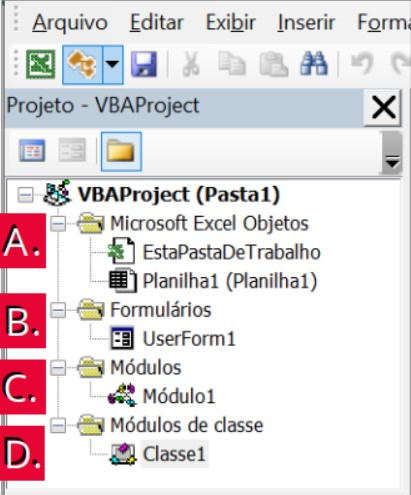
\includegraphics[scale = 0.75]{Screenshot_1.jpg}
    \caption{Interface Básica do VBA}
\end{figure}

\section{Paradigma}
    \begin{itemize}
        \item \textbf{Objetos:} são as estruturas de dados que existem no Excel, com as quais podemos interagir. Ex: Células, Planilhas etc. Ex: Range("A1").
        \item \textbf{Atributos ou Propriedades:} são as características de determinado objeto. Ex: Range("A1").Value 
        \item \textbf{Métodos:} são funções aplicáveis somente àquele objeto
        Range("A1").Clear
        \item \textbf{Parâmetros:} são os parâmetros a serem designados aos métodos para interagir com os objetos. Ex: 
        ThisWorkbook.PrintOut From:=1, To:=2
        \item \textbf{Eventos:} interação do usuário que executa o código.
    \end{itemize}
    
\section{Atalhos}
    \begin{itemize}
        \item Alt + F11: Abre a tela do VBA
        \item F1: Excel VBA Help
        \item F5: Executa o código inteiro
        \item F8: Executa o código linha por linha
        \item Ctrl + Spacebar: Ferramenta de autocompletar códigos
        \item Ctrl + R: Exibe o Project Explorer, onde estão os arquivos contidos naquele VBA Project
    \end{itemize}

\section{Operações Lógicas}

    Executam blocos de código caso uma condição seja verdadeira 

Exemplo:

\begin{lstlisting}[language = VBScript]
    If condicao1 Then
        ...
    ElseIf condicao2 Then
        ...
    Else
        ...
    End If
\end{lstlisting}

\section{Objetos Importantes}
    \subsection{Range}
        Permite manipular uma célula ou coleção de células em uma planilha.
        Exemplos:
        \begin{itemize}
            \item Range("A1")
            \item Range("B2:D3")
            \item Range("B:B")
            \item Range("Célula Nomeada")
        \end{itemize}
        
        \textbf{Observação.:} o método Offset é muito interessante para a manipulação de planilhas, pois permite que o usuário localize uma célula com base na célula ativa. Funciona como um plano cartesiano orientado pelo segundo quadrante, logo números negativos se referem ao lado contrário.
        
        Exemplo: ActiveCell.Offset(1,1).Select -> seleciona a coluna situada a uma linha e uma coluna de distância. 
        
    \subsection{ActiveCell}
        Referência Simples à célula ativa. Outros Exemplos: ThisWorkbook. 
    \subsection{Sheets}
        Referência simples à uma planilha
        Exemplo:
            Sheets("Plan1")



\section{UserForms}
    São caixas de diálogo que permitem a comunicação com o usuário. Podemos inserir um script nos botões de um formulário por exemplo, permitindo que o usuário execute tarefas. 

\newpage
\begin{figure}[h]
    \centering
    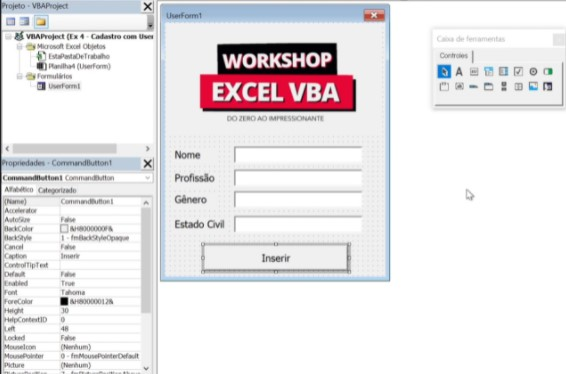
\includegraphics[scale = 0.75]{Screenshot_2.jpg}
    \caption{Exemplo da edição de um Formulário}
\end{figure}
    
\section{Loops}
    Executam um bloco de código enquanto a condição for verdadeira.

    Exemplo:

\begin{lstlisting}[language = VBScript]
    Do Until condicao1
        ...
    Loop
\end{lstlisting}

\end{document}
